\section{Modeling Data Center Power} 
\label{section:Model}


Our objective is to model total data center power at two granularities: for detailed simulation and for abstract analysis.  Two external factors primarily affect data center power usage: the aggregate load presented to the compute infrastructure and the ambient outside air temperature (outside humidity secondarily affects cooling power as well, but, to limit model complexity, we do not consider it here).  We construct our modeling framework by composing models for the individual data center components.  In our abstract models, we replace key steps that determine the detailed distribution of compute load and heat with simple parametric models that enable reasoning about average behavior.

\begin{table}[t]
\centering
\caption{ \textbf{Variable Definitions.} }
\label{table::VariableDefinitions}
%\begin{tabularx}{\linewidth}{r l r l}
\begin{tabular}{r l r l}
   \toprule
    $U$ & Data Center Utilization  & $T$ & Temperature \\
    $u$ & Component Utilization & $\dot{m}$ & Flow Rate \\
    $\kappa$ & Containment Index & $C_{\mathrm{p}}$ & Heat Capacity \\
    $\ell$ & Load Balancing Coefficient & $N_{\mathrm{Srv}}$ & \# of Servers \\
    $E$ & Heat Transfer Effectiveness & $P$ & Power \\
    $\pi$ & Loss Coefficient & $q$ & Heat \\
    $f$ & Fractional Flow Rate & & \\

    %$T$ & Temperature \\
    %$\dot{m}_{\mathrm{air}}$ & Volumetric Flow Rate of Air \\
    %$C_{\mathrm{p}_{\mathrm{air}}}$ & Specific Heat Capacity of Air \\
    %$\kappa$ & Containment Index \\
    %$E$ & Heat Transfer Effectiveness \\
    %$\dot{m}_{\mathrm{F}}$ & Fractional Volumetric Flow Rate \\
   \bottomrule
  \end{tabular}
  %\end{tabularx}
\end{table}

{\bf Framework.}  We formulate total data center power draw, $P_{\mathrm{Total}}$, as a function of total utilization, \U, and ambient outside temperature, \Toutside.  Figure \ref{figure::DataFlow} illustrates the various intermediary data flows and models necessary to map from \U and \Toutside to $P_{\mathrm{Total}}$. Each box is labeled with a sub-section reference that describes that step of the modeling framework.  In the left column, the power and thermal burden generated by IT equipment is determined by the aggregate compute infrastructure utilization, \U.  On the right, the cooling system consumes power in relation to both the heat generated by IT equipment and the outside air temperature.


{\bf Simulation \& Modeling.} In simulation, we relate each component's utilization (processing demand for servers, current draw for electrical conditioning systems, thermal load for cooling systems, etc.) to its power draw on a component-by-compo\-nent basis.  Hence, simulation requires precise accounting of per-component utilization and the connections between each component.  For servers, this means knowledge of how tasks are assigned to machines; for electrical systems, which servers are connected to each circuit; for cooling systems, how heat and air flow through the physical environment.  We suggest several approaches for deriving these utilizations and coupling the various sub-systems in the context of a data center simulator; we are currently developing such a simulator.

However, for high-level reasoning, it is also useful to model aggregate behavior under typical-case or parametric assumptions on load distribution. Hence, from our detailed models, we construct abstract models that hide details of scheduling and topology.

\begin{figure}[t!]
\centering
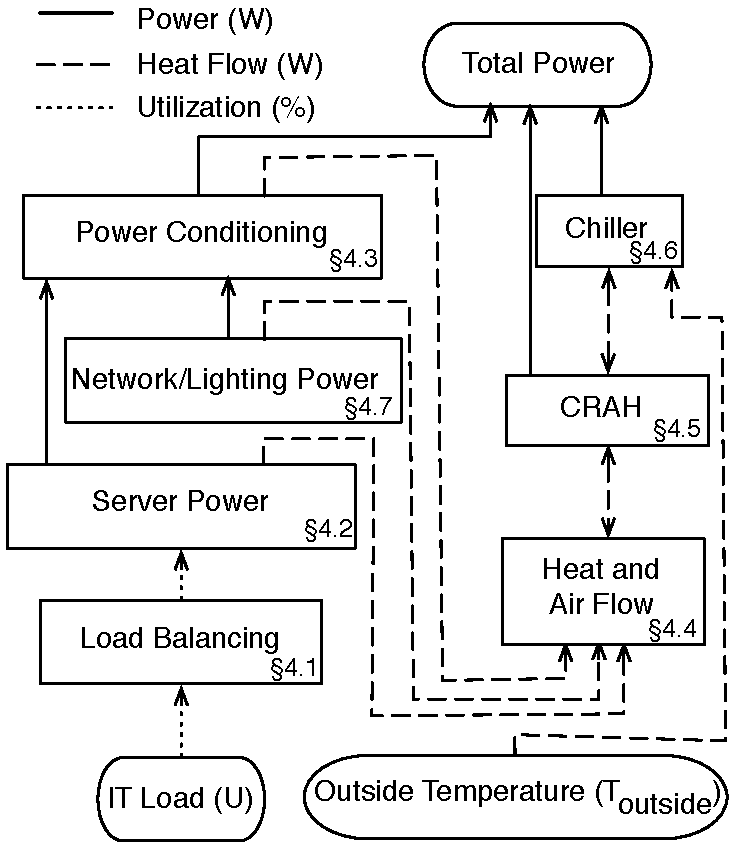
\includegraphics[width = 3 in]{Appendices/WEED/figure/Dependencies.pdf}
\caption{ \textbf{Data Flow.} }
\label{figure::DataFlow}
\end{figure}

{\bf 4.1. Abstracting Server Scheduling.}

The first key challenge in assessing total data center power involves characterizing server utilization and the effects of task scheduling on the power and cooling systems.  Whereas a simulator can incorporate detailed scheduling, task migration, or load balancing mechanisms to derive precise accounting of per-server utilization, we must abstract these mechanisms for analytic modeling.

As a whole, our model relates total data center power draw to aggregate data center utilization, denoted by \U.  Utilization varies from 0 to 1, with 1 representing the peak compute capacity of the data center.  We construe \U as unitless, but it might be expressed in terms of number of servers, peak power (Watts), or compute capability (MIPS).
%Total data center power is the sum of subsystem power draws---servers, power conditioning, cooling, networking, and overhead, each itself a function of \U.
For a given \U, individual server utilizations may vary (e.g., as a function of workload characteristics, consolidation mechanisms, etc.). We represent the per-server utilizations with \usrv, where the subscript indicates the server in question.
For a homogeneous set of  servers:

\begin{equation}
 U = \frac{1}{N_{\mathrm{Srv}}}\sum_{\mathrm{Servers}}u_{\mathrm{Srv}[i]}
\end{equation}

For simplicity, we have restricted our analytic model to a homogeneous cluster.
In real data centers, disparities in performance and power characteristics across servers require detailed simulation to model accurately, and their effect on cooling systems can be difficult to predict \cite{Nathuji08}.

%As we shall see, server power draw is non-linear in \U.  In particular, one might consolidate workloads and turn servers off when \U is low, conserving idle power. Hence, precisely how \U decomposes into per-server power draws is critical to total power requirements.

To abstract the effect of consolidation, we characterize the individual server utilization, \usrv, as a function of \U and a measure of task consolidation, \el.  We use \el to capture the degree to which load is concentrated or spread over the data center's servers. For a given \U and \el we define individual server utilization as:

\begin{equation}
u_{\mathrm{Srv}} = \frac{U}{U + (1-U)\ell}
\end{equation}

\usrv only holds meaning for the $N_{\mathrm{Srv}}(U + (1-U)\ell)$  servers that are non-idle; the remaining servers have zero utilization, and are assumed to be powered off. Figure \ref{figure::ServerUtilization} depicts the relationship among \usrv, \U, and \el.
$\ell = 0$ corresponds to perfect consolidation---the data center's workload is packed onto the minimum number of servers, and the utilization of any active server is 1. $\ell = 1$ represents the opposite extreme of perfect load balancing---all servers are active with \usrv~=~\U.  Varying \el allows us to represent consolidation between these extremes. 

%\begin{figure}[t!]
%  \centering
%  \includegraphics[width = 3.5 in]{figure/LoadBalancingCoeff.pdf}
%  \caption{ \textbf{ Server Utilization. } }
%  \label{figure::ServerUtilization}
%\end{figure}



{\bf 4.2. Server Power.} 

Several studies have characterized server power consumption \cite{BarrosoBook09,Fan07,Meisner09,Rivoire08}.
Whereas the precise shape of the utilization-power relationship varies, servers generally consume roughly half of their peak load power when idle, and power grows with utilization.
In line with prior work \cite{Rivoire08}, we approximate a server's power consumption as linear in utilization between a fixed idle power and peak load power.

\begin{equation}
P_{\mathrm{Srv}} = P_{\mathrm{Srv}_{\mathrm{Idle}}} + ( P_{\mathrm{Srv}_{\mathrm{Peak}}} - P_{\mathrm{Srv}_{\mathrm{Idle}}}) u_{\mathrm{Srv}}
\end{equation}

%In actuality, power draw depends on per-component utilization within the server.  Various components
%exhibit a variety of power to utilization relationships (near constant to quadratic).
%However, CPU utilization is a good approximation for overall system utilization for most workloads  \cite{Rivoire08}.

%\begin{figure}[t!]
%  \centering
%  \includegraphics[width = 3.5 in]{figure/spec.pdf}
%  \caption{ \textbf{ Server Power. } }
%  \label{figure::Spec}
%\end{figure}

Power draw is not precisely linear in utilization; server sub-components exhibit a variety of relationships (near constant to quadratic).
It is possible to use any nonlinear analytical power function, or even a suitable piecewise function.
Additionally, we have chosen to use CPU utilization as an approximation for overal system utilization; a more accurate representation of server utilization might instead be employed.
In simulation, more precise system/workload-specific power modeling is possible by interpolating in a table of measured power values at various utilizations (e.g., as measured with the SpecPower benchmark).
Figure \ref{figure::Spec} compares the linear approximation against published SpecPower results for two recent Dell systems.

{\bf 4.3. Power Conditioning Systems.} 

Data centers require considerable infrastructure simply to distribute uninterrupted, stable electrical power.  PDUs transform the high voltage power distributed throughout the data center to voltage levels appropriate for servers. They incur a constant power loss as well as a power loss proportional to the square of the load \cite{Rasmussen113}:

\begin{equation}
P_{\mathrm{PDU}_{\mathrm{Loss}}} = P_{\mathrm{PDU}_{\mathrm{Idle}}} + \pi_{\mathrm{PDU}}(\sum_{Servers}P_{\mathrm{Srv}})^{2}
\end{equation}

where $P_{\mathrm{PDU}_{\mathrm{Loss}}}$ represents power consumed by the PDU, $\pi_{\mathrm{PDU}}$ represents the PDU power loss coefficient, and $P_{\mathrm{PDU}_{\mathrm{Idle}}}$ the PDU's idle power draw. PDUs typically waste 3\% of their input power.
As current practice requires all PDUs to be active even when idle, the total dynamic power range of PDUs for a given data center utilization is small relative to total data center power; we chose not to introduce a separate PDU load balancing coefficient and instead assume perfect load balancing across all PDUs.

UPSs provide temporary power during utility failures.  UPS systems are typically placed in series between the utility supply and PDUs and impose some power overheads even when operating on utility power.  UPS power overheads follow the relation \cite{Rasmussen113}:

\begin{equation}
P_{\mathrm{UPS}_{\mathrm{Loss}}} = P_{\mathrm{UPS}_{\mathrm{Idle}}} + \pi_{\mathrm{UPS}}\sum_{PDUs}P_{\mathrm{PDU}}
\end{equation}

where $\pi_{\mathrm{UPS}}$ denotes the UPS loss coefficient.  UPS losses typically amount to 9\% of their input power at full load.

%\begin{figure}[t!]
%  \centering
%  \includegraphics[width = 3.5 in]{figure/PowerConditioning.pdf}
%  \caption{ \textbf{ Power Conditioning Losses } }
%  \label{figure::PowerConditioning}
%\end{figure}

%
%\begin{figure*}[ht]
%\centering

%\subfigure[\textbf{ Server Utilization. }]{
%  \includegraphics[width = 2 in]{figure/LoadBalancingCoeff.pdf}
%  \label{figure::ServerUtilization}
%}

%\subfigure[\textbf{ Server Power. } ]{
%  \includegraphics[width = 2 in]{figure/spec.pdf}
%  \label{figure::Spec}
%}

%\subfigure[\textbf{ Power Conditioning Losses }]{
%  \includegraphics[width = 2 in]{figure/PowerConditioning.pdf}
%  \label{figure::PowerConditioning}
%}

%\end{figure*}


\begin{figure*}[ht]

%\begin{minipage}[b]{0.5\linewidth}

\begin{minipage}[b]{.5\linewidth}
  \centering
  \includegraphics[width=\linewidth]{Appendices/WEED/figure/LoadBalancingCoeff.pdf}
  \caption{\textbf{ Individual Server Utilization. }}
  \label{figure::ServerUtilization}
\end{minipage}
\begin{minipage}[b]{0.5\linewidth}
  \centering
  \includegraphics[width = \linewidth]{Appendices/WEED/figure/spec.pdf}
  \caption{\textbf{ Individual Server Power. } }
  \label{figure::Spec}
\end{minipage}
\begin{minipage}[b]{0.5\linewidth}
\centering
  \includegraphics[width = \linewidth]{Appendices/WEED/figure/PowerConditioning.pdf}
\caption{\textbf{ Power Conditioning Losses. }}
  \label{figure::PowerConditioning}
\end{minipage}

\end{figure*}

%Because they are in series, PDU and UPS losses compound.
Figure \ref{figure::PowerConditioning} shows the power losses for a 10MW (peak server power) data center.
At peak load, power conditioning loss is 12\% of total server power.  Furthermore, these losses result in additional heat that must be evacuated by the cooling system.

{\bf 4.4. Heat and Air Flow.} 

Efficient heat transfer in a data center relies heavily on the CRAH's ability to provide servers with cold air.  
CRAHs serve two basic functions: (1) to provide sufficient airflow to prevent recirculation of hot server exhaust to server inlets, and (2) to act as a heat exchanger between server exhaust and some heat sink, typically chilled water.

In general, heat is transferred between two bodies according to the following thermodynamic principle:

\begin{equation}
q = \dot{m} C_{\mathrm{p}} ( T_{\mathrm{h}} - T_{\mathrm{c}})
\end{equation}

Here $q$ is the power transferred between a device and fluid, $\dot{m}$ represents the fluid mass flow, and $C_{\mathrm{p}}$ is the specific heat capacity of the fluid.
$T_{\mathrm{h}}$ and $T_{\mathrm{c}}$ represent the hot and cold temperatures, respectively.
The values of $\dot{m}$, $T_{\mathrm{h}}$, and $T_{\mathrm{c}}$ depend on the physical air flow throughout the data center and air recirculation.

Air recirculation arises when hot and cold air mix before being ingested by servers, requiring a lower cold air temperature and greater mass flow rate to maintain server inlet temperature within a safe operating range.
%Even a small amount of recirculation can require a several degree reduction in CRAH cold-air supply temperature to avoid local hot spots and server overheating.
Data center designers frequently use computational fluid dynamics (CFD) to model the complex flows that arise in a facility and lay out racks and CRAHs to minimize recirculation.  The degree of recirculation depends greatly on data center physical topology, use of containment systems, and the interactions among high-velocity equipment fans.  In  simulation, it is possible to perform CFD analysis to obtain accurate flows. 

For abstract modeling, we replace CFD with a simple parametric model of recirculation that can capture its effect on data center power.  We introduce a \emph{containment index} ($\kappa$), based on previous metrics for recirculation \cite{Tozer09, VanGilder07}.
Containment index is defined as the fraction of air ingested by a server that is supplied by a CRAH (or, at the CRAH, the fraction that comes from server exhaust).
The remaining ingested air is assumed to be recirculated from the device itself.
Thus, a $\kappa$ of 1 implies no recirculation (a.k.a. perfect containment).
Though containment index varies across servers and CRAHs (and may vary with changing airflows), our abstract model uses a single, global containment index to represent average behavior, resulting in the following heat transfer equation:

\begin{equation}
q  = \kappa \dot{m}_{\mathrm{air}} C_{\mathrm{p}_{\mathrm{air}}} ( T_{\mathrm{a}_\mathrm{h}} - T_{\mathrm{a}_\mathrm{c}})
\label{equation::HeatTransfer}
\end{equation}

%\begin{figure}[t!]
%  \centering
%  \includegraphics[width = 3.5 in]{figure/AirFlow1CRAHSupply.pdf}
%  \caption{ \textbf{ Effects of $\kappa$ and u on air flow } }
%  \label{figure::AirFlow}
%\end{figure}
\begin{figure*}[ht]

%\begin{minipage}[b]{0.5\linewidth}

\begin{minipage}[b]{0.5\linewidth}
  \centering
  \includegraphics[width = \linewidth]{Appendices/WEED/figure/AirFlow1CRAHSupply.pdf}
  \caption{ \textbf{ CRAH Supply Temperature. } }
  \label{figure::AirFlow}
\end{minipage}
\begin{minipage}[b]{0.5\linewidth}
\centering
  \includegraphics[width = \linewidth]{Appendices/WEED/figure/CRAH1CI.pdf}
  \caption{ \textbf{ CRAH Power. } }
  \label{figure::CRAH}
\end{minipage}
\begin{minipage}[b]{0.5\linewidth}
  \centering
 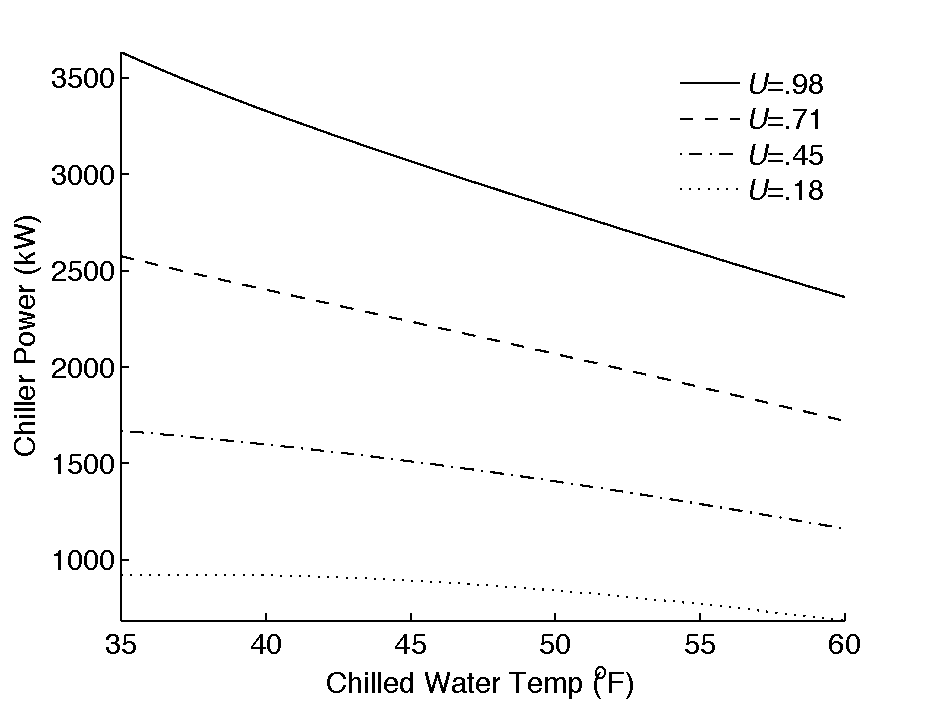
\includegraphics[width = \linewidth]{Appendices/WEED/figure/ChillerCHWSvaryQ.pdf}
   \caption{ \textbf{ Chilled Water Temperature.} }
  \label{figure::ChillerA}
\end{minipage}

\end{figure*}
For this case, $q$ is the heat transferred by the device (either server or CRAH), $\dot{m}_{\mathrm{air}}$ represents the total air flowing through the device, $T_{\mathrm{a}_{\mathrm{h}}}$ the temperature of the air exhausted by the server, and $T_{\mathrm{a}_{\mathrm{c}}}$ is the temperature of the cold air supplied by the CRAH.  These temperatures represent the hottest and coldest air temperatures in the system, respectively, and are not necessarily the inlet temperatures observed at servers and CRAHs (except for the case when $\kappa = 1$).

Using only a single value for $\kappa$ simplifies the model by allowing us to enforce the conservation of air flow between the CRAH and servers.
Figure \ref{figure::AirFlow} demonstrates the burden air recirculation places on the cooling system. We assume flow through a server increases linearly with server utilization (representing variable-speed fans) and a peak server power of 200 watts.
The left figure shows the CRAH supply temperature necessary to maintain the typical maximum safe server inlet temperature of 77$^{\circ}$F.  As $\kappa$ decreases, the required CRAH supply temperature quickly drops.  Moreover, required supply temperature drops faster as utilization approaches peak.  As we show next, lowering supply temperature results in super-linear increases in CRAH and chiller plant power.
Preventing air recirculation (e.g., with containment systems) can drastically improve cooling efficiency.

{\bf 4.5. Computer Room Air Handler.} 

CRAHs transfer heat out of the server room to the chilled water loop.  We model this exchange of heat using a modified effectiveness-NTU method \cite{Cengel03}:

\begin{equation}
q_{\mathrm{crah}} = E \, \kappa  \,\dot{m}_{\mathrm{air}} C_{\mathrm{p}_\mathrm{air}} f^{0.7} (\kappa \, T_{\mathrm{a}_\mathrm{h}} + (1-\kappa) T_{\mathrm{a}_\mathrm{c}} - T_{\mathrm{w}_\mathrm{c}})
\end{equation}

$q_{\mathrm{crah}}$ is the heat removed by the CRAH, $E$ is the transfer efficiency at the maximum mass flow rate (0 to 1), $f$ represents the volume flow rate as a fraction of the maximum volume flow rate, and $T_{\mathrm{w}_\mathrm{c}}$ the chilled water temperature.

CRAH power is dominated by fan power, which grows with the cube of mass flow rate to some maximum, here denoted as $P_{\mathrm{CRAH}_{\mathrm{Dyn}}}$.
Additionally, there is some fixed power cost for sensors and control systems, $P_{\mathrm{CRAH}_{\mathrm{Idle}}}$.  We model CRAH units with variable speed drives (VSD) that allow volume flow rate to vary from zero (at idle) to the CRAH's peak volume flow.  Some CRAH units are cooled by air rather than chilled water or contain other features such as humidification systems which we do not consider here.

\begin{equation}
P_{\mathrm{CRAH}} = P_{\mathrm{CRAH}_{\mathrm{Idle}}} +  P_{\mathrm{CRAH}_{\mathrm{Dyn}}} f^3
\end{equation}

As the volume flow rate through the CRAH increases, both the mass available to transport heat and the efficiency of heat exchange increase. This increased heat transfer efficiency somewhat offsets the cubic growth of fan power as a function of air flow.  The true relationship between CRAH power and heat removed falls between a quadratic and cubic curve.
Additionally, the CRAH's ability to remove heat depends on the temperature difference between the CRAH air inlet and water inlet. Reducing recirculation and lowering the chilled water supply temperature reduce the power required by the CRAH unit.% (though lower chilled water supply temperature implies higher power cost at the chiller plant). 




%\begin{figure}[t!]
%  \centering
%  \includegraphics[width = 3.5 in]{figure/CRAH1CI.pdf}
%  \caption{ \textbf{ Effects of $\kappa$, U, and Chiller Water Supply Temperature on CRAH Power. } }
%  \label{figure::CRAH}
%\end{figure}

The effects of containment index and chilled water supply temperature on CRAH power are shown in Figure \ref{figure::CRAH}. Here the CRAH model has a peak heat transfer efficiency of 0.5, a maximum airflow of 6900 CFM, peak fan power of 3kW, and an idle power cost of 0.1 kW.  When the chilled water supply temperature is low, CRAH units are relatively insensitive to changes in containment index.
For this reason data center operators often choose low chilled water supply temperature, leading to overprovisioned cooling in the common case.

{\bf 4.6. Chiller Plant and Cooling Tower.} 

The chiller plant provides a supply of chilled water or glycol, removing heat from the warm water return.
Using a compressor, this heat is transferred to a second water loop, where it is pumped to an external cooling tower.  The chiller plant's compressor accounts for the majority of the overall cooling cost in most data centers.  Its power draw depends on the amount of heat extracted from the chilled water return, the selected temperature of the chilled water supply, the water flow rate, the outside temperature, and the outside humidity.  For simplicity, we neglect the effects of humidity.  In current-generation data centers, the water flow rate and chilled water supply temperature are held constant during operation (though there is substantial opportunity to improve cooling efficiency with variable-temperature chilled water supply).

Numerous chiller types exist, typically classified by their compressor type.  The HVAC community has developed several modeling approaches to assess chiller performance. Although physics-based models do exist, we chose the Department of Energy's DOE2 chiller model \cite{DOE2}, an empirical model comprising a series of regression curves.  Fitting the DOE2 model to a particular chiller requires numerous physical measurements.  Instead, we use a benchmark set of regression curves provided by the California Energy Commission \cite{CEC}. We do not detail the DOE2 model here, as it is well documented and offers little insight into chiller operation.  We neglect detailed modeling of the cooling tower, using outside air temperature as a proxy for cooling tower water return temperature.

As an example, a chiller at a constant outside temperature and chilled water supply temperature will require power that grows quadratically with the quantity of heat removed (and thus with utilization).  A chiller intended to remove 8MW of heat at peak load using 3,200 kW at a steady outside air temperature of 85$^{\circ}$F, a steady chilled water supply temperature of 45$^{\circ}$F, and a data center load balancing coefficient of 0 (complete consolidation) will consume the following power as a function of total data center utilization (kW):

$$P_{\mathrm{Chiller}} = 742.8 U^{2} + 1,\!844.6 U + 538.7$$

\begin{figure*}[ht]
\begin{minipage}[b]{0.5\linewidth}
\centering
    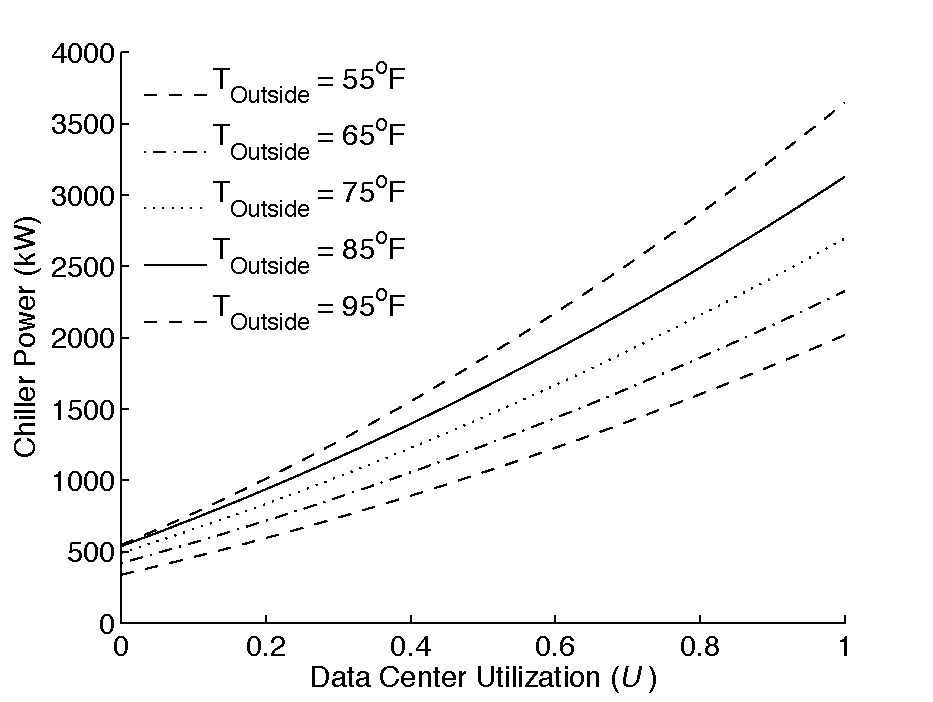
\includegraphics[width = \linewidth]{Appendices/WEED/figure/ChillerLoadvaryOutside.pdf}
  \caption{\textbf{ Effects of $U$ and $T_{\mathrm{Outside}}$ on $P_{\mathrm{Chiller}}$ } }
  \label{figure::ChillerB}
  \end{minipage}
  \hspace{0.5cm}
  \begin{minipage}[b]{0.5\linewidth}
\centering
    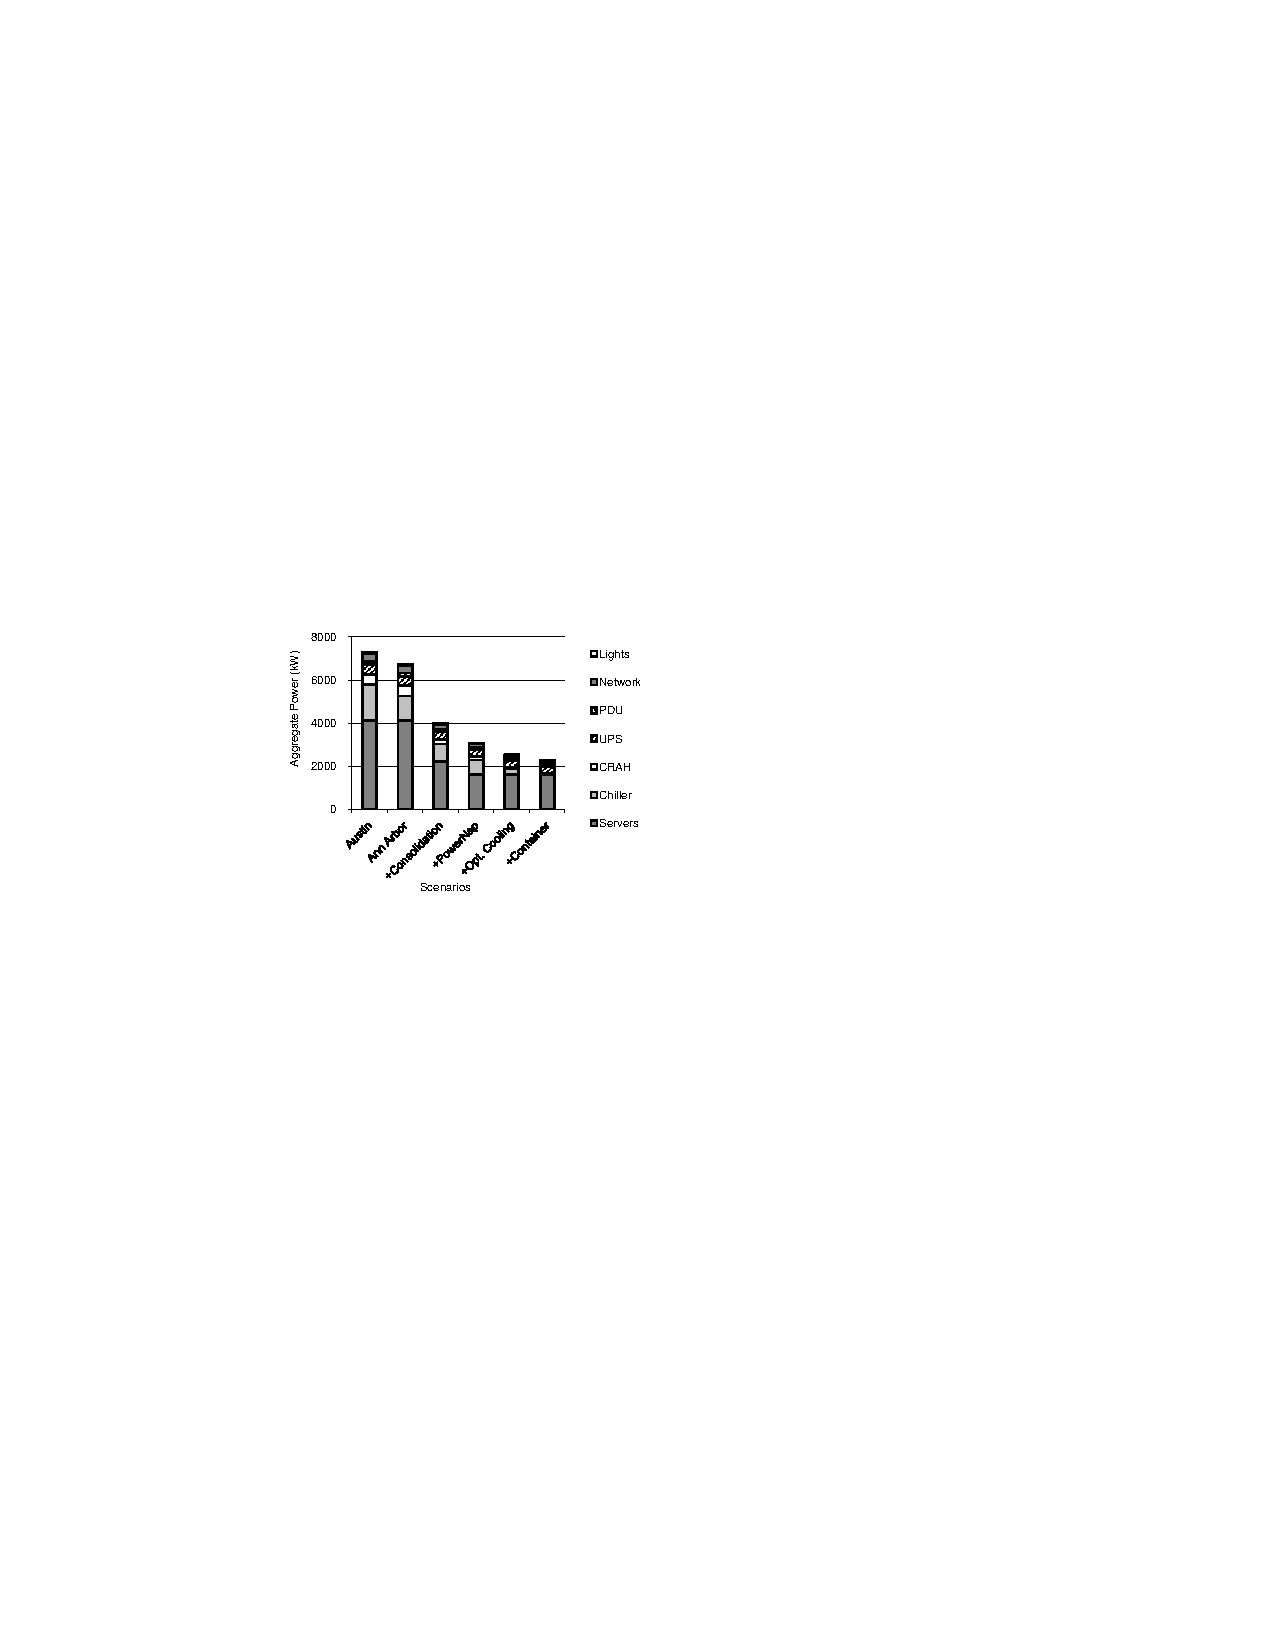
\includegraphics[width = \linewidth]{Appendices/WEED/figure/comparison.pdf}
  \caption{\textbf{ A Case Study of Power-Saving Features.} }
  \label{figure::comparison}
  \end{minipage}

\end{figure*}

Figure \ref{figure::ChillerA} demonstrates the power required to supply successively lower chilled water temperatures at various \U for an 8MW peak thermal load.
When thermal load is light, chiller power is relatively insensitive to chilled water temperature, which suggests using a conservative (low) set point to improve CRAH efficiency.  
However, as thermal load increases, the power required to lower the chilled water temperature becomes substantial.
The difference in chiller power for a 45$^{\circ}$F and 55$^{\circ}$F chilled water supply at peak load is nearly 500kW.
Figure \ref{figure::ChillerB} displays the rapidly growing power requirement as the cooling load increases for a 45$^{\circ}$F chilled water supply.
The graph also shows the strong sensitivity of chiller power to outside air temperature.

{\bf 4.7. Miscellaneous Power Draws.} 

Networking equipment, pumps, and lighting all contribute to total data center power.  However, the contribution of each is quite small (a few percent). None of these systems have power draws that vary significantly with data center load.  We account for these subsystems by including a term for fixed power overheads (around 6\% of peak) in the overall power model.  We do not currently consider the impact of humidification within our models.

{\bf 4.8. Applying the Model: A Case Study.} 

To demonstrate the utility of our abstract models, we contrast the power requirements of several hypothetical data centers.  Each scenario builds on the previous, introducing a new power-saving feature. We analyze each data center at 25\% utilization.
Table \ref{table::MockDataCenters} lists our scenarios and Figure \ref{figure::comparison} displays their respective power draws.
\begin{table}[b]
\begin{center}
%\footnotesize
\caption{ \textbf{Hypothetical Data Centers.} }
\label{table::MockDataCenters}
%\begin{tabularx}{\linewidth}{l l l l l l}
\begin{tabular}{l l l l l l}
   \toprule
      Data Center & $\ell$ & $\kappa$ & $\frac{P_{\mathrm{Idle}}}{P_{\mathrm{Peak}}}$ & $T (F)$ & Opt. Cooling \\
    \midrule
      Austin & .95 & .9 & .6 & 70 & no \\
      Ann Arbor & .95 & .9 & .6 & 50 & no \\
      +Consolidation & .25 & .9 & .6 & 50 & no \\
      +PowerNap & .25 & .9 & .05 & 50 & no \\
      +Opt. Cooling & .25 & .9 & .05 & 50 & yes \\
      +Containers & .25 & .99 & .05 & 50 & yes \\
  \bottomrule
  %\end{tabularx}
  \end{tabular}
\end{center}
\end{table}
\emph{Austin} and \emph{Ann Arbor} represent conventional data centers with legacy physical infrastructure typical of facilities commissioned in the last three to five years.  We use yearly averages for outside air temperature (reported in $^{\circ}$F).  We assume limited server consolidation and a relatively poor (though not atypical) containment index of 0.9. Furthermore, we assume typical (inefficient) servers with idle power at 60\% of peak power, and static chilled water and CRAH air supply temperatures set to 45$^{\circ}$F and 65$^{\circ}$F, respectively.  We scale the data centers such that the Austin facility consumes precisely 10MW at peak utilization. With the exception of \emph{Austin}, all data centers are located in Ann Arbor.

The outside air temperature difference between \emph{Austin} and \emph{Ann Arbor} yields substantial savings in chiller power.  Note, however, that aggregate data center power is dominated by server power, nearly all of which is wasted by idle systems.  \emph{Consolidation} represents a data center where virtual machine consolidation or other mechanisms reduce \el  from 0.95 to 0.25, increasing individual server utilization from 0.26 to 0.57 and reducing the number of active servers from 81\% to 44\%.
Improved consolidation drastically decreases aggregate power draw, but, paradoxically, it increases power usage effectiveness (PUE; total data center power divided by IT equipment power).  These results illustrate the shortcoming of PUE as a metric for energy efficiency---it fails to account for the (in)effi\-ciency of IT equipment.  \emph{PowerNap} \cite{Meisner09} allows servers to idle at 5\% of peak power by transitioning rapidly to a low power sleep state, reducing overall data center power another 22\%.  PowerNap and virtual machine consolidation take alternative approaches to target the same source of energy inefficiency: server idle power waste.

The \emph{Optimal Cooling} scenario posits integrated, dynamic control of the cooling infrastructure.
We assume an optimizer with global knowledge of data center load/environmental conditions that seeks to minimize chiller power.  The optimizer chooses the highest $T_{\mathrm{w}_\mathrm{c}}$ that still allows CRAHs to meet the maximum allowable server inlet temperature. 
This scenario demonstrates the potential for intelligent cooling management.  Finally, \emph{Container} represents a data center with a containment system (e.g., servers enclosed in shipping containers), where containment index is increased to 0.99.  Under this scenario, the cooling system power draw is drastically reduced and power conditioning infrastructure becomes the limiting factor on power efficiency.

%In a real data center, this optimization requires precise server inlet tracking and prediction of the optimal chilled water supply temperature, along with mechanisms to coordinate chiller operation.  

%\vspace{-.25 in}
%$$q_{\mathrm{crac}} = S \rho CFM \cdot C_{\mathrm{p}_\mathrm{a}} (T_{\mathrm{a}_\mathrm{h}} - T_{\mathrm{a}_\mathrm{c}})$$
%\vspace{-.25 in}
%
%\vspace{-.25 in}
%$$T_{\mathrm{a}_\mathrm{h}} = \frac{T_{\mathrm{a}_\mathrm{c}} - \tilde{E}(\frac{CFM_{\mathrm{crac}}}{CFM_{\mathrm{max}}})^{.7} T_{\mathrm{w}_\mathrm{c}}  }{ 1 - \tilde{E} (\frac{CFM_{\mathrm{crac}}}{CFM_{\mathrm{max}}})^{.7}  } $$
%\vspace{-.25 in}
%
%\vspace{-.25 in}
%$$CFM_{\mathrm{server}} = \frac{q_{\mathrm{total}}}{S \rho C_{\mathrm{p}_{\mathrm{air}}} (T_{\mathrm{a}_\mathrm{h}} - T_{\mathrm{a}_\mathrm{c}}) } $$
%\vspace{-.25 in}
%
%$\dot{m}_{\mathrm{crac}} =S \dot{m}_{\mathrm{server}}$, S = Number of servers assigned to CRAC
%
%$q_{\mathrm{CRAC}} = S q_{\mathrm{server}}$, $\dot{m} = \rho CFM$
%
%Effectiveness NTU
%
%$q = \epsilon \dot{m} C_\mathrm{p} (T_{\mathrm{h}_\mathrm{i}} - T_{\mathrm{c}_\mathrm{i}})$
%
%{\bf Pump.}
%
%Total Dynamic Head
%
%\vspace{-.25 in}
%$$TDH = H_{\mathrm{pipping}} + H_{\mathrm{tower}} + H_{\mathrm{condenser}} $$
%\vspace{-.25 in}
%
%\vspace{-.25 in}
%$$H_{\mathrm{pipping}} = (\frac{S^2}{2g} )(\frac{F \cdot L_{\mathrm{eq}}}{d} )$$
%\vspace{-.25 in}
%
%
%$S$ = Fluid Velocity, $f$ = friction factor
%$g$ = gravity, $h_{eq}$ = equivalent length of straight pipe
%$d$ = pipe diameter
%
%
%\vspace{-.25 in}
%$$F = \frac{1}{( -1.8 \log( \frac{6.9}{\Re_\mathrm{d}} + ( \frac{\varepsilon_\mathrm{p}}{d 3.7})^{1.11} ) )^2 }$$
%\vspace{-.25 in}
%
%$\eta$ = pump efficiency
%
%\vspace{-.25 in}
%$$P_{\mathrm{pump}} = (\frac{ gpm \cdot TDH}{3960 \cdot \eta_{\mathrm{pump}} })$$
%\vspace{-.25 in}
%
%$\eta_{\mathrm{motor}}$ = motor efficiency
%
%
%\vspace{-.25 in}
%$$P_{\mathrm{motor}} = (\frac{P_{\mathrm{pump}} }{\eta_{\mathrm{motor}} })$$
%\vspace{-.25 in}


